\subsection{Entity-Relationship Schema}

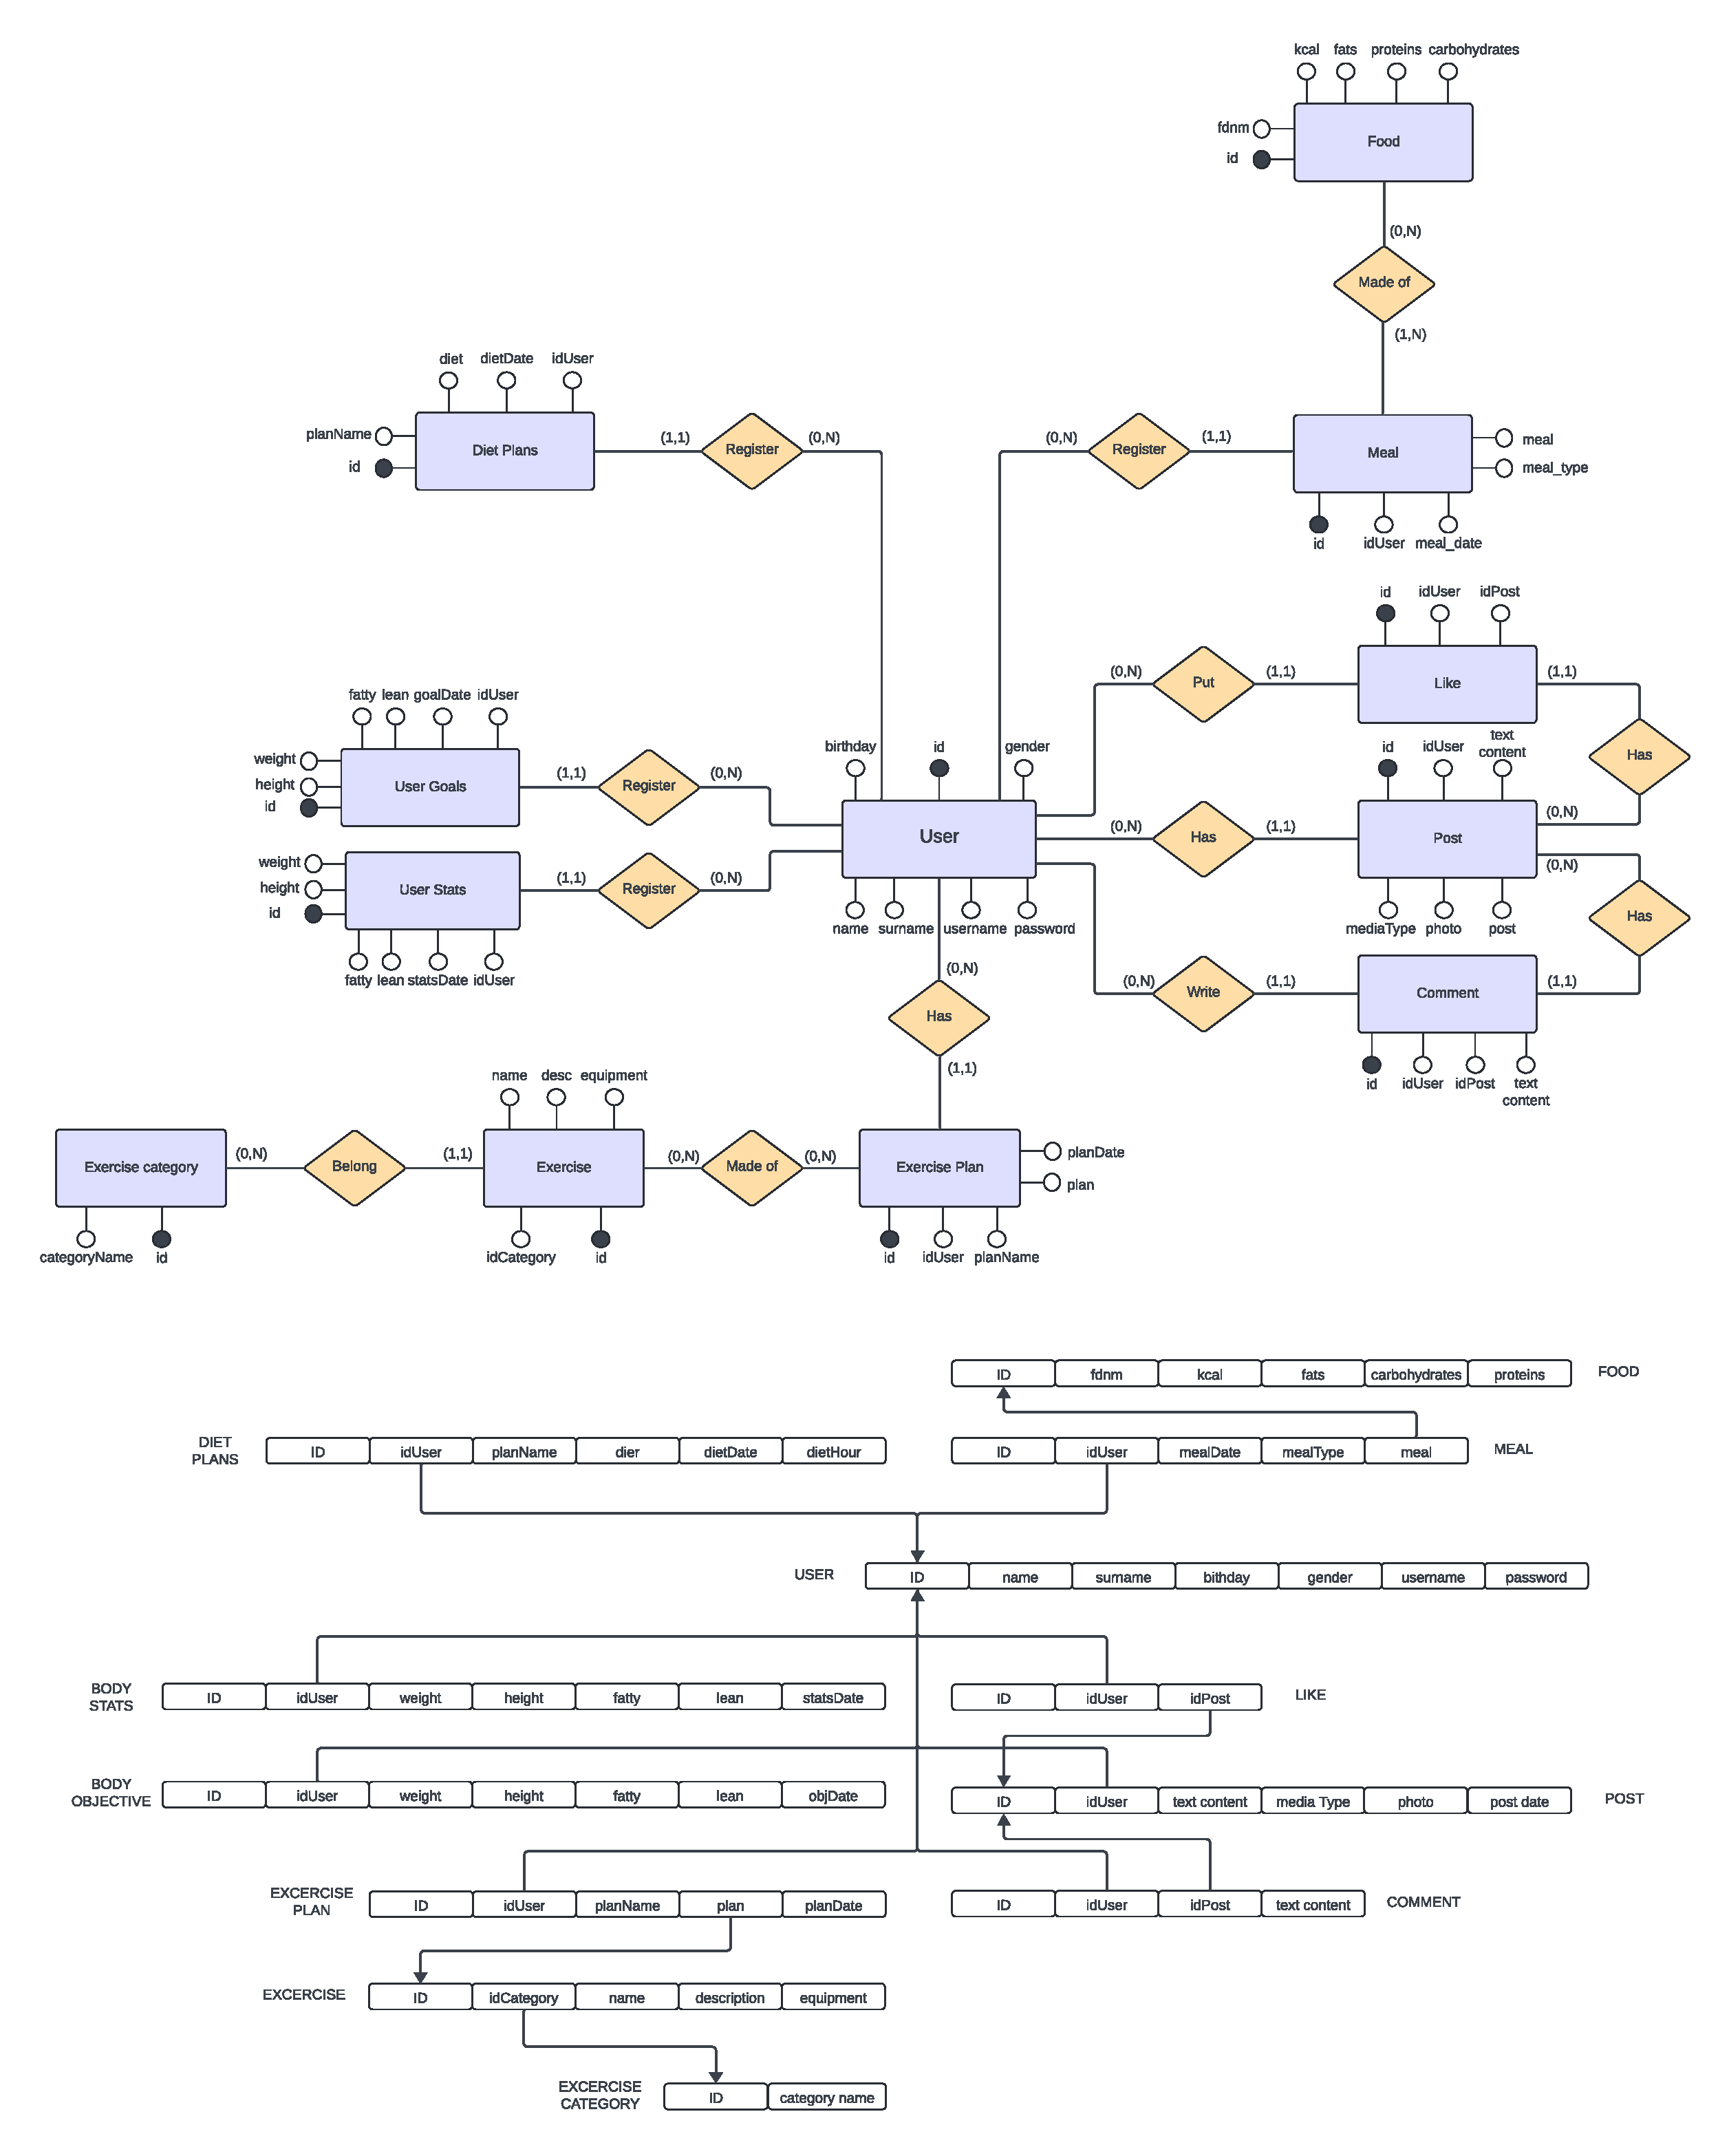
\includegraphics[scale=0.38]{Resources/ER.pdf}

\newpage
%Describe here your ER schema
\begin{itemize}
    \item \textbf{User}: Each user of the application is identified by an ID (type of INT). For each user we also save
their Name, Surname, gender, username and password as VARCHAR and birthday of type DATE. The primary key is the ID and we have the constraint UNIQUE for the username field.
    \item \textbf{User Stats}: Contains all records of user's body statistics measures of weight,height, lean and fatty mass. The primary key is the ID but have a unique constraint on idUser and Date that allows the user to insert at most one measures per day.
    \item \textbf{User Goals}: Contains the same field and constraint of the User Stats table but is intended to keep track of user's goals.
    \item \textbf{Posts}: Contains all the posts of the social network. Each post belongs to a specific user and is made of text and eventually a photo and characterized by the timestamp of it's creation. Photos are saved in the DB as Byte type. Primary key is the ID.  
    \item \textbf{Likes}: Contains the all the likes for the posts of the social network, each one characterized by the user id of the user who liked the post and the id of the post liked. Constraint on user Id and postId allows user to create only one like per post. Primary key is the ID.
    \item \textbf{Comments}: Contains all the comments, made of text, of the social network, each one characterized by the id of the user who commented the post and the id of the post commented. Primary key is the ID. 
    \item \textbf{Diet Plans}: Contains all informations about the diet of the user: planName, dietDate and the entire diet. The primary key is the ID but have a unique constraint on idUser and dietDate that allows the user to change a diet within the first 24 hours of adding it-
    \item \textbf{Meal}: Contains the records of the meals of the user. The primary key is the ID, but has a unique constraint on idUser, date of the meal and the type of the meal: a user can have a type of meal once a day (one breakfast, one lunch, etc). In addition to these fields, the table contains the string with the single meal.
    \item \textbf{Food}: Contains the list of the foods registered. The primary key is the ID. The other fields are the stats for 100g of the food.
    \item \textbf{Exercise Plan}: Contains all the exercises of the user which are: planName, planDate and the entire plan (which is the exercise plans of the user). The primary Key is the ID.
    \item \textbf{Exercise}: Contains the list of the exercises. The primary key is the ID. it has idCategory as a foreign key and also shows the name of the exercise and a description about it and the equipment that are needed for doing the exercise.
    \item \textbf{Exercise Category}: Contains the list of the exercise categories. the primary key is the ID.
\end{itemize}